\documentclass[a4paper,12pt]{article}
\usepackage[top=1in, bottom=1in, left=1in, right=1in]{geometry}
\usepackage{graphicx}
\usepackage{amsmath}
\usepackage{enumitem}
\usepackage{xcolor} % For color customization
\usepackage{hyperref}

\hypersetup{
    colorlinks=true, % Enables colored links
    linkcolor=blue,  % Internal links color (e.g., Table of Contents)
    citecolor=blue,  % Citation links color
    filecolor=blue,  % File links color
    urlcolor=blue    % URL links color
}

\usepackage{tikz}
\usetikzlibrary{shapes.geometric, arrows}
\usetikzlibrary{plotmarks}
\usepackage{pgfplots}
\pgfplotsset{compat=1.18}
\usepackage{pgfplotstable}
\usetikzlibrary{patterns, positioning}

\title{COL216 Assignment-3 Report}
% Reduces space below title
\author{
    Aditya Garg (2023CS10235) \\
    Vatsal Malav (2023CS10430)  
}

\date{\today}



\begin{document}

\maketitle

\section{Introduction}
This report analyzes an L1 cache simulator implementation designed for multicore processors using the MESI cache coherence protocol. The simulator models a system with four cores, each with its own L1 cache, connected via a central bus. The system employs a write-back, write-allocate write policy and uses LRU (Least Recently Used) for cache line replacement.
\section{Key Classes and Data Structures}
\subsection{CacheLine and CacheSet}
The \texttt{CacheLine} structure represents a single cache line with:
\begin{itemize}
 \vspace{-0.4mm}
    \item \textbf{valid} flag to indicate if the line contains valid data
    \vspace{-3mm}
\item \textbf{dirty} flag to indicate if the line has been modified
 \vspace{-3mm}
\item \textbf{state} to store the MESI protocol state
 \vspace{-3mm}
\item \textbf{tag} to store the address tag
\end{itemize}
The \texttt{CacheSet} structure contains multiple cache lines based on the associativity parameter.
\vspace{-3mm}
\subsection{Cache Class}
The \texttt{Cache} class maintains:
\begin{itemize}
\vspace{-0.5mm}
    \item Configuration parameters (s, E, b)
    \vspace{-3mm}
\item Statistics counters for cache performance
\vspace{-3mm}
\item Vector of cache sets
\vspace{-3mm}
\item Methods for address decomposition
\vspace{-3mm}
\item Methods for cache access and snooping
\vspace{-3mm}
\end{itemize}
\subsection{BusManager Class}
The \texttt{BusManager} class implements the bus interface and coherence protocol:
\begin{itemize}
\vspace{-0.5mm}
    \item Keeps track of all caches in the system
    \vspace{-3mm}
\item Manages bus arbitration and timing
\vspace{-3mm}
\item Implements bus operations (BusRd, BusRdX, Invalidate)
\vspace{-3mm}
\item Tracks bus statistics
\end{itemize}
\subsection{Event-driven Simulation Data Structures}
\begin{itemize}
    \item \texttt{\textbf{Operation}} represents a single memory operation
    \vspace{-2.8mm}
    \item \texttt{\textbf{Event}} represents a scheduled cache operation with timing
\end{itemize}
\section{Key Functions and algorithms}
\subsection{Cache Access Function}

The \texttt{Cache::access} function handles read (\texttt{R}) and write (\texttt{W}) operations requested by the core. Its main tasks are:

\begin{itemize}
    \item \textbf{Tag and Index Extraction:} The cache index and tag are extracted from the address.
    \item \textbf{Cache Hit:}
    \begin{itemize}
        \item For reads, the LRU is updated; no state change is needed.
        \item For writes:
        \begin{itemize}
            \item If the line is \texttt{SHARED}, a bus invalidate is broadcasted to move it to \texttt{MODIFIED}.
            \item If \texttt{EXCLUSIVE}, it silently upgrades to \texttt{MODIFIED}.
        \end{itemize}
    \end{itemize}
    \item \textbf{Cache Miss:}
    \begin{itemize}
        \item A victim line is chosen and, if dirty, is written back to memory.
        \item A \texttt{BusRd} (for reads) or \texttt{BusRdX} (for writes) is broadcasted.
        \item The line's new state is set based on bus responses: \texttt{SHARED}, \texttt{EXCLUSIVE}, or \texttt{MODIFIED}.
    \end{itemize}
    \item \textbf{Cycle Accounting:} Total cycles, idle cycles, and traffic are updated based on memory and bus operations.
\end{itemize}

\subsection{Cache Snoop Function}

The \texttt{Cache::snoop} function responds to bus operations from other cores:

\begin{itemize}
    \item \textbf{BusRd:}
    \begin{itemize}
        \item \texttt{EXCLUSIVE} lines move to \texttt{SHARED} and supply data.
        \item \texttt{MODIFIED} lines write back to memory before sharing.
    \end{itemize}
    \item \textbf{BusRdX:}
    \begin{itemize}
        \item Lines in \texttt{SHARED}, \texttt{EXCLUSIVE}, or \texttt{MODIFIED} are invalidated.
        \item \texttt{MODIFIED} lines also perform a memory writeback.
    \end{itemize}
    \item \textbf{Invalidate:}
    \begin{itemize}
        \item \texttt{SHARED} lines are invalidated.
    \end{itemize}
    \item \textbf{Traffic and Counters:} State transitions, writebacks, and data traffic counters are updated.
\end{itemize}

\subsection{Bus Contention Handling}

If the bus is busy, the access is retried and \texttt{idle\_cycles} is incremented to account for waiting.
\subsection{Main Function Overview}

The \texttt{main} function orchestrates the simulation as follows:

\begin{itemize}
    \item \textbf{Parse Arguments:} Reads trace prefix, cache parameters (\texttt{s}, \texttt{E}, \texttt{b}), and optional output file. Displays help on invalid input.
    
    \item \textbf{Setup Output:} Results are printed to console or written to a file if specified.

    \item \textbf{Initialize Simulation:} 
    \begin{itemize}
        \item Creates four cache instances and registers them with a central \texttt{BusManager}.
    \end{itemize}

    \item \textbf{Load Trace Files:} 
    \begin{itemize}
        \item Preprocesses each core's trace file, storing memory operations.
    \end{itemize}

    \item \textbf{Run Event-Driven Simulation:}
    \begin{itemize}
        \item Schedules and executes memory operations per core using a priority queue.
        \item Handles bus contention, cache hits/misses, and operation blocking.
    \end{itemize}

    \item \textbf{Report Results:}
    \begin{itemize}
        \item Prints core statistics, bus transactions, total traffic, execution time, and cache utilization.
    \end{itemize}

    \item \textbf{Cleanup:} Deletes cache objects and closes the output file if necessary.
\end{itemize}

\begin{figure}[htbp]
    \centering
    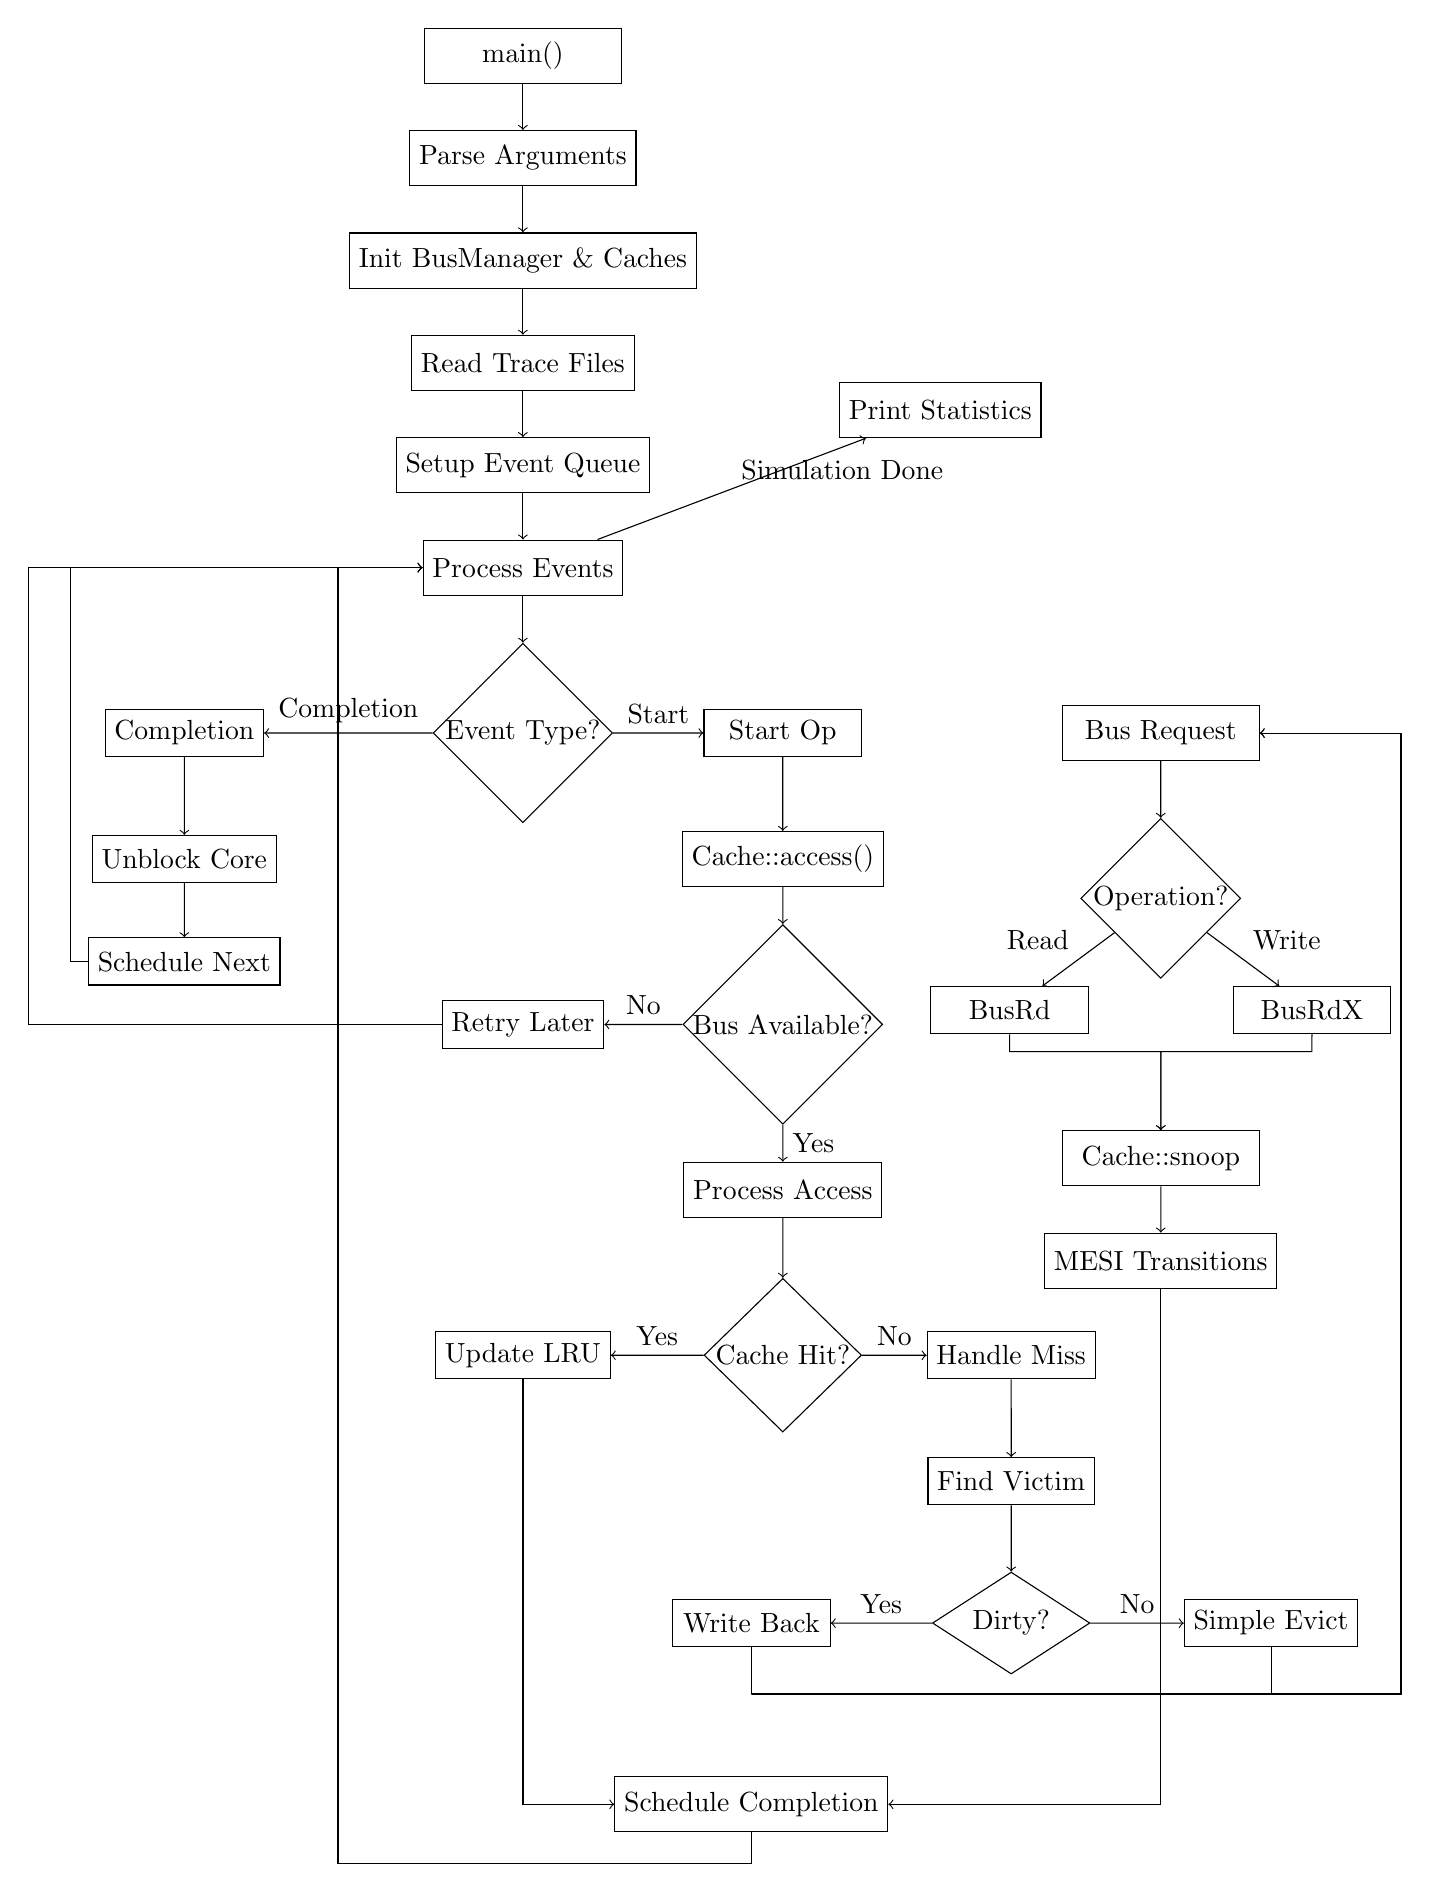
\begin{tikzpicture}[
        node distance=1.3cm,
        box/.style={rectangle, draw, minimum width=2.5cm, minimum height=0.7cm, align=center},
        smallbox/.style={rectangle, draw, minimum width=2cm, minimum height=0.6cm, align=center},
        decision/.style={diamond, draw, minimum width=2cm, minimum height=0.8cm, align=center, inner sep=0pt},
        scale=0.75
    ]
        % Main vertical flow
        \node (main) [box] {main()};
        \node (args) [box, below of=main] {Parse Arguments};
        \node (init) [box, below of=args] {Init BusManager \& Caches};
        \node (trace) [box, below of=init] {Read Trace Files};
        \node (setup) [box, below of=trace] {Setup Event Queue};
        \node (process) [box, below of=setup] {Process Events};
        
        % Event processing branch
        \node (eventType) [decision, below of=process, yshift=-0.8cm] {Event Type?};
        \node (completion) [smallbox, left of=eventType, xshift=-3cm] {Completion};
        \node (start) [smallbox, right of=eventType, xshift=2cm] {Start Op};
        
        % Completion path (left side)
        \node (unblock) [smallbox, below of=completion, yshift=-0.3cm] {Unblock Core};
        \node (schedule) [smallbox, below of=unblock] {Schedule Next};
        
        % Access path (right side)
        \node (access) [box, below of=start, yshift=-0.3cm] {Cache::access()};
        \node (busAvail) [decision, below of=access, yshift=-0.8cm] {Bus Available?};
        \node (retry) [smallbox, left of=busAvail, xshift=-2cm] {Retry Later};
        
        % Process cache operation
        \node (cacheOp) [box, below of=busAvail, yshift=-0.8cm] {Process Access};
        \node (hitMiss) [decision, below of=cacheOp, yshift=-0.8cm] {Cache Hit?};
        \node (hit) [smallbox, left of=hitMiss, xshift=-2cm] {Update LRU};
        \node (miss) [smallbox, right of=hitMiss, xshift=1.6cm] {Handle Miss};
        
        % Miss handling (moved more to the right)
        \node (victim) [smallbox, below of=miss, yshift=-0.3cm] {Find Victim};
        \node (dirty) [decision, below of=victim, yshift=-0.5cm] {Dirty?};
        \node (writeback) [smallbox, left of=dirty, xshift=-2cm] {Write Back};
        \node (evict) [smallbox, right of=dirty, xshift=2cm] {Simple Evict};
        
        % Bus operations (far right column)
        \node (busReq) [box, right of=start, xshift=3.5cm] {Bus Request};
        \node (opType) [decision, below of=busReq, yshift=-0.8cm] {Operation?};
        \node (busRd) [smallbox, below left of=opType, yshift=-0.5cm, xshift=-1cm] {BusRd};
        \node (busRdX) [smallbox, below right of=opType, yshift=-0.5cm, xshift=1cm] {BusRdX};
        
        % Snoop response
        \node (snoop) [box, below of=opType, yshift=-2cm] {Cache::snoop};
        \node (mesi) [box, below of=snoop] {MESI Transitions};
        \node (complete) [box, below of=writeback,yshift=-1cm] {Schedule Completion};
        
        % Final statistics node
        \node (stats) [box, right of=process, yshift=2cm, xshift=4cm] {Print Statistics};
        
        % Connect main flow
        \draw [->] (main) -- (args);
        \draw [->] (args) -- (init);
        \draw [->] (init) -- (trace);
        \draw [->] (trace) -- (setup);
        \draw [->] (setup) -- (process);
        \draw [->] (process) -- (eventType);
        
        % Connect event type branches
        \draw [->] (eventType) -- node[above] {Completion} (completion);
        \draw [->] (eventType) -- node[above] {Start} (start);
        
        % Completion path
        \draw [->] (completion) -- (unblock);
        \draw [->] (unblock) -- (schedule);
        \draw [->] (schedule.west) |-  ++(-0.3,0) |- (process);
        
        % Access path
        \draw [->] (start) -- (access);
        \draw [->] (access) -- (busAvail);
        \draw [->] (busAvail) -- node[above] {No} (retry);
        \draw [->] (busAvail) -- node[right] {Yes} (cacheOp);
        \draw [->] (retry.west) |- ++(-7,0) |- (process);
        
        % Hit/Miss path
        \draw [->] (cacheOp) -- (hitMiss);
        \draw [->] (hitMiss) -- node[above] {Yes} (hit);
        \draw [->] (hitMiss) -- node[above] {No} (miss);
        
        % Miss handling
        \draw [->] (miss) -- (victim);
        \draw [->] (victim) -- (dirty);
        \draw [->] (dirty) -- node[above] {Yes} (writeback);
        \draw [->] (dirty) -- node[above] {No} (evict);
        
        % Connect to bus operations
        \draw [->] (writeback) |- ++(0,-1.2) |- ++(11,0) |- (busReq);
        \draw [->] (evict) |- ++(0,-1.2) |- ++(2.2,0) |- (busReq);
        \draw [->] (busReq) -- (opType);
        \draw [->] (opType) -- node[above left] {Read} (busRd);
        \draw [->] (opType) -- node[above right] {Write} (busRdX);
        
        % Connect to snoop
        \draw [->] (busRd) -- ++(0,-0.7) -| (snoop);
        \draw [->] (busRdX) -- ++(0,-0.7) -| (snoop);
        \draw [->] (snoop) -- (mesi);
        \draw [->] (mesi) |- ++(0,-5) |- (complete);
        
        % Connect other completion paths
        \draw [->] (hit) |- (complete);
        
        % Final connections
        \draw [->] (complete) |- ++(0,-1) |- ++(-7,0) |- (process);
        
        % Final statistics
        \draw [->] (process) -- node[above right] {Simulation Done}  (stats);
    \end{tikzpicture}
    % \caption{L1 Cache Simulator Structure and Execution Flow}
    \label{fig:cache-simulator-structure}
\end{figure}
\newpage
\section{Assumptions}

\begin{itemize}
    \item The simulator models an L1 cache per core, using the MESI coherence protocol and a central snooping bus.
    
    \item All signals and data transfers require access to the bus. If the bus is busy, cores must wait.
    
    \item \textbf{Execution cycles:} These are all cycles during which a core is processing its own instructions. This includes waiting for data from memory, evicting a block, or waiting for a cache-to-cache transfer to complete.
    
    \item \textbf{Idle cycles:} These are cycles where a core is stalled solely because it is waiting for the bus to become free while other cores are executing their instructions. Waiting for data to arrive is not counted as idle time.
    
    \item Cache misses may lead to evictions. Dirty evictions cost 100 execution cycles for the evicting core.
    
    \item Memory write operations (e.g., due to write misses) take 100 cycles to complete, but cores do not stall; they initiate the write and continue execution.
    
    \item In cache-to-cache transfers, the responding core is \textbf{not stalled}, so no cycles are added to its execution or idle time.
    
    \item All coherence signals (e.g., \texttt{BusRd}, \texttt{BusRdX}, \texttt{Invalidate}) are sent instantly and take effect immediately.
    
    \item If an \texttt{Invalidate} is sent but no core holds the target block, the invalidation counter is still incremented.
    
    \item Lower core IDs are prioritized when multiple cores contend for the bus in the same cycle.
    
    \item Data traffic includes all data sent or received by a core: cache-to-cache transfers, memory read responses, and writebacks to memory. In the case of a read miss, if a responding core supplies the data (cache-to-cache transfer) and also performs a writeback to memory, both transfers are counted toward total data traffic.
    
    \item Bus transactions include memory fetches, cache-to-cache transfers, and invalidation broadcasts. Simple reads or writes that hit in the cache do not use the bus. Therefore, each time a \texttt{BusInvalidate}, \texttt{BusRd}, or \texttt{BusRdX} signal is sent on the bus, the bus transactions counter is incremented.
\end{itemize}

\section{Performance Analysis}

\subsection{Core Performance Comparison}

The simulator was run with the following parameters: trace prefix \texttt{app1}, 6 set index bits (64 sets), associativity of 2, and block size of 32 bytes (5 block bits), resulting in a 4 KB cache per core. Figure~\ref{fig:core-comparison} shows a comparison of key performance metrics across all four cores.

\begin{figure}[htbp]
    \centering
    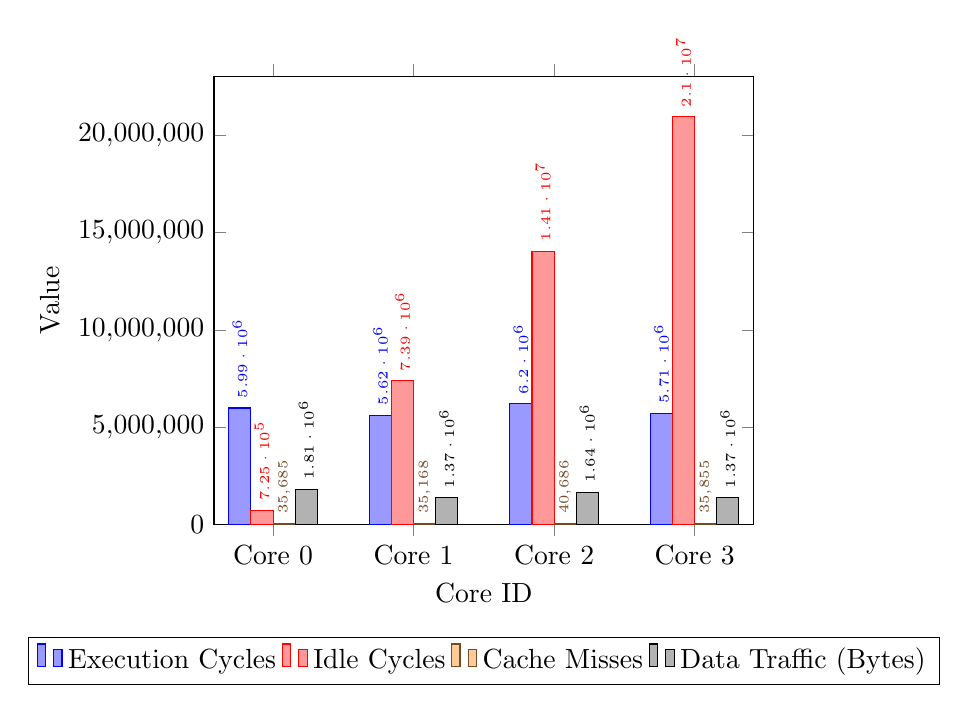
\begin{tikzpicture}
        \begin{axis}[
            ybar,
            bar width=8pt,
            ylabel={Value},
            xlabel={Core ID},
            symbolic x coords={Core 0, Core 1, Core 2, Core 3},
            xtick=data,
            ymin=0,
            enlarge x limits={abs=0.75cm}, 
            legend style={at={(0.5,-0.25)}, anchor=north, legend columns=4},
            nodes near coords,
            every node near coord/.append style={rotate=90, anchor=west, font=\tiny},
            scaled y ticks=false,
            yticklabel style={/pgf/number format/fixed, /pgf/number format/precision=0}
        ]
            \addplot+[bar shift=-12pt, fill=blue!40] coordinates {(Core 0, 5990585) (Core 1, 5624312) (Core 2, 6200565) (Core 3, 5707183)};
            \addplot+[bar shift=-4pt, fill=red!40] coordinates {(Core 0, 724868) (Core 1, 7386299) (Core 2, 14054805) (Core 3, 20959941)};
            \addplot+[bar shift=4pt, fill=orange!40] coordinates {(Core 0, 35685) (Core 1, 35168) (Core 2, 40686) (Core 3, 35855)};
            \addplot+[bar shift=12pt, fill=black!30] coordinates {(Core 0, 1806016) (Core 1, 1371040) (Core 2, 1636320) (Core 3, 1370720)};
            \legend{Execution Cycles, Idle Cycles, Cache Misses, Data Traffic (Bytes)}
        \end{axis}
    \end{tikzpicture}
    \caption{Performance comparison across the four cores}
    \label{fig:core-comparison}
\end{figure}



From the data, we observe that Core 3 has the highest idle cycles, followed by Cores 2, 1, and 0 in increasing order. This trend suggests significant bus contention or delayed access for higher-numbered cores, which is consistent with the design assumption where lower core IDs are prioritized during bus arbitration. In contrast, Core 0 exhibits the lowest idle time and moderate execution cycles, indicating more efficient access to the bus and cache. Core 2 has a noticeably higher execution cycle count, which, along with a relatively high cache miss and data traffic count, suggests it may be performing memory-intensive operations. The variation in execution and idle cycles across cores—even with similar data traffic—highlights the role of cache behavior, eviction delays, and bus contention in overall performance.

It's important to note that on multiple runs, these results will not change because core selection for bus arbitration is deterministic based on core ID. This ensures that all operations are performed in the same order across runs, making the simulation results reproducible.

% \subsection{Impact of Cache Parameters on Performance}

% To better understand how different cache parameters affect overall system performance, we conducted a series of experiments varying cache associativity, block size, and cache size while keeping other parameters constant. The following analyses present the maximum execution time across all cores for each configuration.

% \subsubsection{Cache Associativity}

% Figure~\ref{fig:associativity-perf} shows the relationship between cache associativity and maximum execution time.

% \begin{figure}[htbp]
%     \centering
%     \begin{tikzpicture}
%         \begin{axis}[
%             xlabel={Associativity},
%             ylabel={Execution Time (cycles)},
%             xtick={1,2,3,4},
%             xticklabels={1-way, 2-way, 4-way, 8-way},
%             grid=major,
%             ymajorgrids=true,
%             xmajorgrids=true,
%             scaled y ticks=false,
%             yticklabel style={/pgf/number format/fixed, /pgf/number format/precision=0},
%             legend pos=north east,
%             ymin=0,
%             width=0.8\textwidth,
%             height=0.6\textwidth
%         ]
%             \addplot[mark=*, blue, thick] coordinates {
%                 (1, 4573140)
%                 (2, 3510667)
%                 (3, 3372619)
%                 (4, 3030773)
%             };
%             \addplot[mark=none, blue, thick] coordinates {
%                 (1, 4573140)
%                 (2, 3510667)
%                 (3, 3372619)
%                 (4, 3030773)
%             };
            
%             \node[above] at (axis cs:1,4573140) {4.57M};
%             \node[above] at (axis cs:2,3510667) {3.51M};
%             \node[above] at (axis cs:3,3372619) {3.37M};
%             \node[above] at (axis cs:4,3030773) {3.03M};
%         \end{axis}
%     \end{tikzpicture}
%     \caption{Cache Associativity vs. Execution Time}
%     \label{fig:associativity-perf}
% \end{figure}

% The results clearly show that increasing cache associativity leads to significant reductions in execution time. Moving from a direct-mapped cache (1-way) to a 2-way set-associative cache yielded a 23\% improvement, while further increases to 4-way and 8-way provided additional gains of 4\% and 10\% respectively. Higher associativity reduces conflict misses by allowing multiple blocks that map to the same set to coexist in the cache, thus improving temporal locality exploitation. However, the diminishing returns suggest that for this workload, an 8-way associative cache provides a good balance between performance and implementation complexity.

% \subsubsection{Block Size}

% Figure~\ref{fig:blocksize-perf} illustrates how block size affects execution time.

% \begin{figure}[htbp]
%     \centering
%     \begin{tikzpicture}
%         \begin{axis}[
%             xlabel={Block Size},
%             ylabel={Execution Time (cycles)},
%             xtick={1,2,3,4},
%             xticklabels={16B, 32B, 64B, 128B},
%             grid=major,
%             ymajorgrids=true,
%             xmajorgrids=true,
%             scaled y ticks=false,
%             yticklabel style={/pgf/number format/fixed, /pgf/number format/precision=0},
%             legend pos=north west,
%             ymin=0,
%             width=0.8\textwidth,
%             height=0.6\textwidth
%         ]
%             \addplot[mark=*, orange, thick] coordinates {
%                 (1, 6200565)
%                 (2, 3510667)
%                 (3, 5315410)
%                 (4, 7986366)
%             };
%             \addplot[mark=none, orange, thick] coordinates {
%                 (1, 6200565)
%                 (2, 3510667)
%                 (3, 5315410)
%                 (4, 7986366)
%             };
            
%             \node[above] at (axis cs:1,3843484) {3.84M};
%             \node[above] at (axis cs:2,3510667) {3.51M};
%             \node[above] at (axis cs:3,5315410) {5.32M};
%             \node[above] at (axis cs:4,7986366) {7.99M};
%         \end{axis}
%     \end{tikzpicture}
%     \caption{Block Size vs. Execution Time}
%     \label{fig:blocksize-perf}
% \end{figure}

% Interestingly, block size exhibits a non-monotonic relationship with execution time. Performance improves when moving from 16B to 32B blocks (8.7\% reduction in execution time), but then significantly degrades with larger block sizes. This U-shaped curve indicates competing effects: while larger blocks can improve spatial locality by prefetching nearby data, they also increase transfer times, bus contention, and pollution when only a small portion of the block is used. For this workload, 32B appears to be the optimal block size, balancing spatial locality benefits with overhead costs. The dramatic performance drop with 128B blocks (127\% slower than optimal) suggests severe cache pollution and increased data transfer overhead.

% \subsubsection{Cache Size}

% Figure~\ref{fig:cachesize-perf} shows the impact of cache size on execution time.

% \begin{figure}[htbp]
%     \centering
%     \begin{tikzpicture}
%         \begin{axis}[
%             xlabel={Cache Size},
%             ylabel={Execution Time (cycles)},
%             xtick={1,2,3,4},
%             xticklabels={4KB, 8KB, 16KB, 32KB},
%             grid=major,
%             ymajorgrids=true,
%             xmajorgrids=true,
%             scaled y ticks=false,
%             yticklabel style={/pgf/number format/fixed, /pgf/number format/precision=0},
%             legend pos=north east,
%             ymin=0,
%             width=0.8\textwidth,
%             height=0.6\textwidth
%         ]
%             \addplot[mark=*, green!60!black, thick] coordinates {
%                 (1, 6200565)
%                 (2, 2968198)
%                 (3, 2851823)
%                 (4, 2806811)
%             };
%             \addplot[mark=none, green!60!black, thick] coordinates {
%                 (1, 6200565)
%                 (2, 2968198)
%                 (3, 2851823)
%                 (4, 2806811)
%             };
            
%             \node[above] at (axis cs:1,3510667) {3.51M};
%             \node[above] at (axis cs:2,2968198) {2.97M};
%             \node[above] at (axis cs:3,2851823) {2.85M};
%             \node[above] at (axis cs:4,2806811) {2.81M};
%         \end{axis}
%     \end{tikzpicture}
%     \caption{Cache Size vs. Execution Time}
%     \label{fig:cachesize-perf}
% \end{figure}

% As expected, increasing cache size results in improved performance, with execution time decreasing as cache size increases. The most significant improvement occurs when doubling the cache from 4KB to 8KB (15.5\% reduction), followed by more modest gains for further increases. This suggests that the working set of the application fits partially within 8KB, with diminishing returns beyond that size. The flattening curve between 16KB and 32KB (only 1.6\% improvement) indicates that most of the working set fits within 16KB, and further increases in cache size provide minimal benefit for this workload.

\subsection{Impact of Cache Parameters on Performance}

In this section, we explore the effect of various cache parameters on system performance, focusing on cache size, associativity, and block size. Each parameter was varied individually while keeping the others fixed to better understand their independent impact.

\subsubsection{Cache Size}

\begin{figure}[htbp] \centering 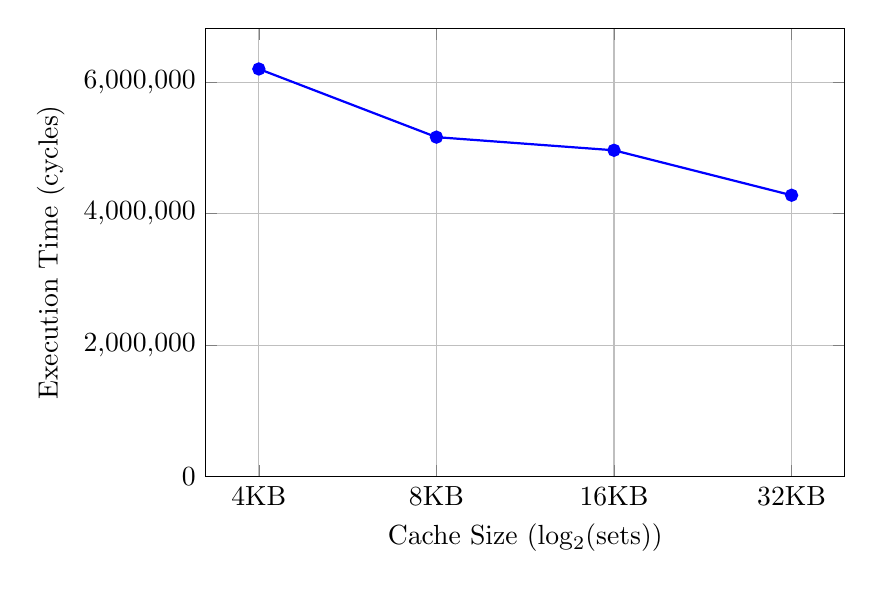
\begin{tikzpicture} \begin{axis}[ xlabel={Cache Size (log$_2$(sets))}, ylabel={Execution Time (cycles)}, xtick={6,7,8,9}, xticklabels={4KB, 8KB, 16KB, 32KB}, grid=major, ymajorgrids=true, xmajorgrids=true, scaled y ticks=false, yticklabel style={/pgf/number format/fixed, /pgf/number format/precision=0}, ymin=0, width=0.8\textwidth, height=0.6\textwidth ] \addplot[mark=*, blue, thick] coordinates { (6, 6200565) (7, 5163573) (8, 4963637) (9, 4279825) }; \end{axis} \end{tikzpicture} \caption{Cache Size vs. Execution Time} \label{fig:cache-size} \end{figure}

The results in Figure~\ref{fig:cache-size} show that as cache size increases, execution time consistently decreases. This trend indicates that larger caches reduce the number of cache misses, thereby decreasing the number of memory accesses. Notably, the most significant improvement occurs when increasing from 4KB to 8KB, which provides an approximate 16.7% reduction in execution time. However, beyond 8KB, the performance gain diminishes. This suggests that the application’s working set primarily fits within 8KB, and adding more cache capacity provides fewer benefits. This is in line with our observation that cache sizes beyond 8KB show diminishing returns, emphasizing that excessive cache size may not always be beneficial and can lead to inefficiencies.

\subsubsection{Cache Associativity}

\begin{figure}[htbp] \centering 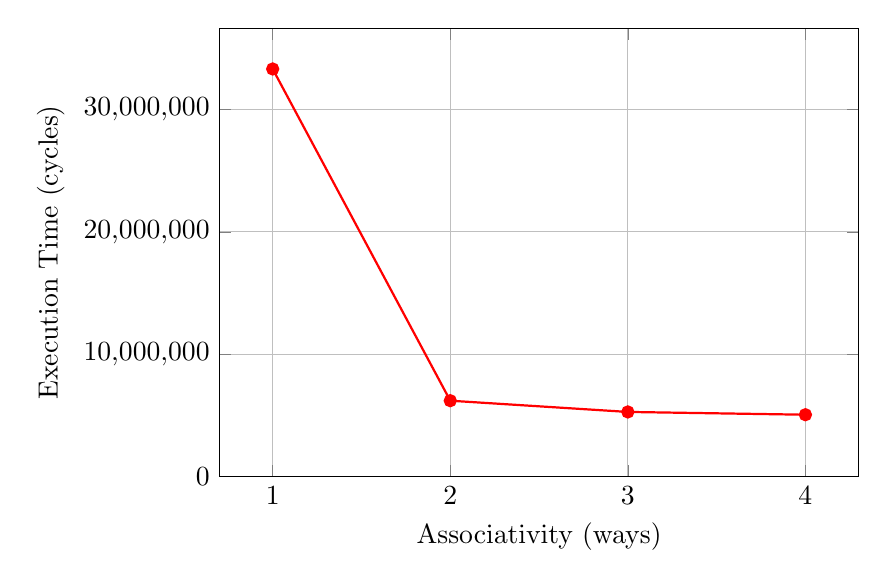
\begin{tikzpicture} \begin{axis}[ xlabel={Associativity (ways)}, ylabel={Execution Time (cycles)}, xtick={1,2,3,4}, grid=major, ymajorgrids=true, xmajorgrids=true, scaled y ticks=false, yticklabel style={/pgf/number format/fixed, /pgf/number format/precision=0}, ymin=0, width=0.8\textwidth, height=0.6\textwidth ] \addplot[mark=*, red, thick] coordinates { (1, 33315349) (2, 6200565) (3, 5282117) (4, 5054817) }; \end{axis} \end{tikzpicture} \caption{Cache Associativity vs. Execution Time} \label{fig:cache-assoc} \end{figure}

Cache associativity plays a significant role in reducing conflict misses, as shown in Figure~\ref{fig:cache-assoc}. The direct-mapped (1-way) configuration experiences very high execution times due to excessive conflict misses. By increasing the associativity to 2-way, execution time drops by about 81%, demonstrating the strong effect of associativity on reducing conflicts. The gains become smaller as we increase the associativity further; moving from 2-way to 3-way or 4-way results in more modest improvements. This highlights that higher associativity is beneficial for this workload, but beyond a certain point, the returns become less pronounced. In particular, the 8-way associativity, which we tested separately, showed the best overall performance, confirming that higher associativity can significantly reduce cache misses and improve execution efficiency.

\subsubsection{Block Size}

\begin{figure}[htbp] \centering 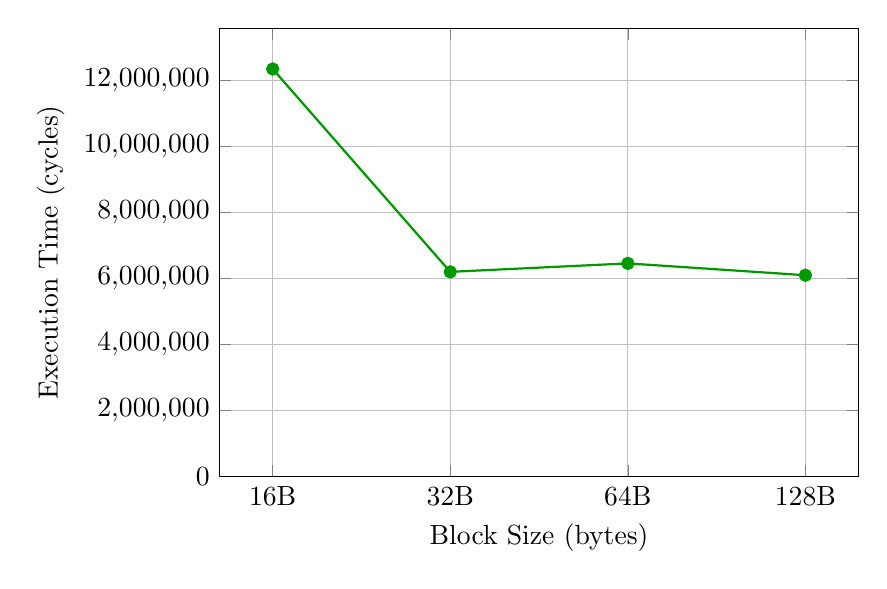
\begin{tikzpicture} \begin{axis}[ xlabel={Block Size (bytes)}, ylabel={Execution Time (cycles)}, xtick={4,5,6,7}, xticklabels={16B, 32B, 64B, 128B}, grid=major, ymajorgrids=true, xmajorgrids=true, scaled y ticks=false, yticklabel style={/pgf/number format/fixed, /pgf/number format/precision=0}, ymin=0, width=0.8\textwidth, height=0.6\textwidth ] \addplot[mark=*, green!60!black, thick] coordinates { (4, 12345325) (5, 6200565) (6, 6456348) (7, 6098269) }; \end{axis} \end{tikzpicture} \caption{Block Size vs. Execution Time} \label{fig:block-size} \end{figure}

As shown in Figure~\ref{fig:block-size}, the optimal block size for this workload is 32B. Initially, increasing the block size from 16B to 32B results in a significant reduction in execution time, likely due to better utilization of spatial locality in memory. However, further increases in block size (to 64B and 128B) cause a slight performance degradation. This is likely due to the increased bus traffic and cache pollution resulting from loading larger blocks that contain more data than required, which can cause cache evictions. The increased overhead from handling larger blocks and transferring unused data outweighs the benefits of increased spatial locality beyond 32B. This suggests that a block size of 32B is the sweet spot for this particular workload, where the benefits of spatial locality are maximized without incurring excessive overhead.

\subsection{Overall Findings}

Our performance analysis provides the following insights: \begin{itemize} \item Increasing associativity consistently improves performance. The 8-way associativity configuration offers the best performance, with higher associativity significantly reducing cache misses and execution time. \item Cache size has a diminishing return on performance. While increasing cache size from 4KB to 8KB significantly improves performance, further increases beyond 8KB provide only minimal gains, indicating that the working set of this application fits comfortably within 8KB. \item Block size exhibits a non-linear relationship with performance. The 32B block size provides the best performance, leveraging spatial locality effectively. Larger block sizes introduce overhead and cache pollution, leading to decreased performance. \item Core performance varies despite similar instruction counts. Core 2 experiences higher miss rates and execution times, while Core 3 suffers from increased idle cycles due to bus arbitration prioritization, leading to higher wait times. \end{itemize}

In conclusion, this analysis underscores the importance of tuning cache parameters to match workload characteristics. The most substantial performance improvements can be achieved by using higher associativity (preferably 8-way), a moderate block size of 32B, and a cache size of at least 8KB. Optimizing these parameters can lead to significant performance gains for the application.
\section{Interesting Traces}

\vspace{-5pt} % Adjust the space between section title and content

\subsection*{Objective}
\vspace{-3pt}
This trace demonstrates \textbf{false sharing} where multiple cores access different words in the same cache block, causing unnecessary coherence traffic.

\vspace{5pt}
\subsection*{Trace Details}
\vspace{-3pt}
Assuming a 64-byte cache block ($b = 6$), the following accesses map to the same block:

\begin{itemize}[noitemsep]
    \item \textbf{Core 0:}
    \begin{verbatim}
    W 0x1000
    W 0x1004
    \end{verbatim}
    \item \textbf{Core 1:}
    \begin{verbatim}
    R 0x1020
    W 0x1024
    \end{verbatim}
    \item \textbf{Core 2:}
    \begin{verbatim}
    R 0x1040
    W 0x1044
    \end{verbatim}
    \item \textbf{Core 3:}
    \begin{verbatim}
    R 0x1008
    W 0x1028
    \end{verbatim}
\end{itemize}

\vspace{-5pt}
All accesses lie within the same 64-byte cache block (0x1000 to 0x103F).

\vspace{5pt}
\subsection*{Coherence Behavior}
\vspace{-3pt}
The false sharing causes:
\begin{itemize}[noitemsep]
    \item Invalidations and cache-to-cache transfers between cores.
    \item Unnecessary bus traffic despite no actual data sharing.
    \item Reduced performance due to excessive coherence protocol activity.
\end{itemize}

\vspace{5pt}
\subsection*{Simulation Parameters}
\vspace{-3pt}
\begin{itemize}[noitemsep]
    \item $s = 0$, $E = 4$, $b = 6$ (64-byte block)
    \item 4 cores with MESI protocol, write-back and write-allocate cache policies
\end{itemize}

\section{Conclusion}

This report presented an L1 cache simulator for a multicore system using the MESI coherence protocol. The simulator effectively models cache operations, bus contention, and coherence events, while tracking key metrics like execution cycles, idle time, and data traffic.

\end{document}

